\newpage

\chapter{Реализация}
\label{ch:chapter_2}

\section{Выбор технологий для реализации сетевой архитектуры}

\subsection{Детальная проработка требований}
\label{sec:detailed_requirements}
Существует множество способов установить сетевое взаимодействие между
приложениями, начиная от низкоуровневой обработки пакетов на уровне стека
TCP/IP, заканчивая использованием высокоуровневых объектно-ориентированных
библиотек для протоколов прикладного уровня. Был сформирован ряд ограничений
(см. главу \ref{sec:problem_statement}), которых необходимо придерживаться при
выборе технологии для построения сетевой архитектуры.

В соответствии с концепцией сетевого взаимодействия (см. главу
\ref{sec:collaborative_mindmapping}), мы имеем клиент-серверную архитектуру.
Взаимодействие пользователей будет более удобным, если сервер можно будет
создавать на любом устройстве и в любой момент времени. Взаимодействие должно
выглядеть следующим образом: пользователь создаёт сервер, другие участники
подсоединяются к нему и начинают редактирование. Каждое изменение, сделанное
участником, отправляется на сервер, который рассылает это изменение всем другим
участникам (см. рис. \ref{img:users_collaboration_example}). Для надежного
сообщения между клиентами и сервером, все участники должны иметь одинаковую и верную копию карты.

\begin{figure}[!h]
  \centering
  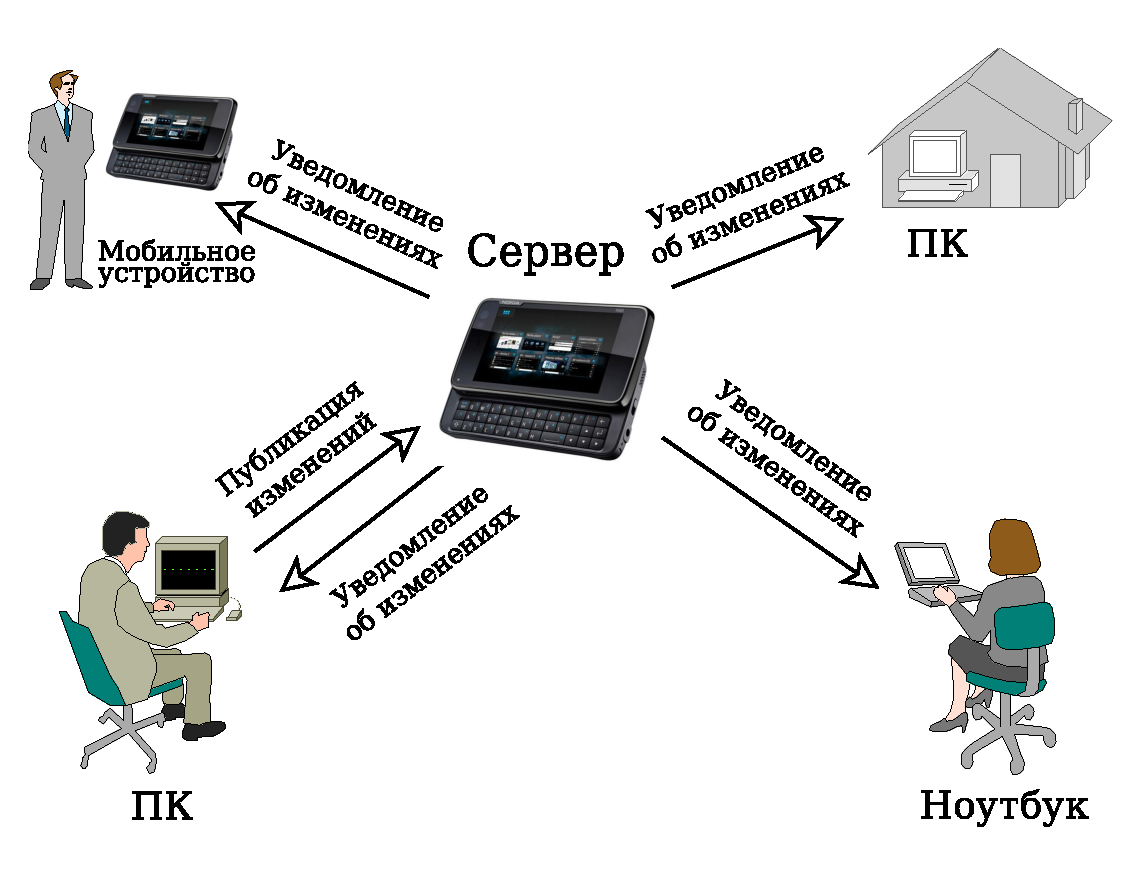
\includegraphics[width=\linewidth]{users_collaboration_example.pdf}
  \caption{Взаимодействие клиентов и сервера}
  \label{img:users_collaboration_example}
\end{figure} 

Проект HiveMind поддерживает мобильные устройства и настольные компьютеры (см.
главу \ref{sec:project_summary}), имеющие различный способ подключения к
интернету. У каждого из этих способов есть свои преимущества и
недостатки. Пользователи настольных компьютеров, как правило, имеют широкий
канал интернет соединения, в отличие от пользователей мобильных устройств.
Мобильные устройства способны подключаться к интернету почти везде и в любое
время. В связи с нехваткой IPv4 адресов, операторы мобильной связи назначают
серые ip адреса мобильным устройствам, что делает данные устройства недоступными
напрямую из сети Интернет. Соединение по беспроводным сетям зачастую нестабильно
и иногда вызывает значительные задержки при передачи данных. Пользователи
настольных компьютеров могут использовать NAT или фаервол блокирующий
входящие соединения. В корпоративной среде, пользователи зачастую ограничены
HTTP прокси, как единственным способом доступа в сеть Интернет.

Подводя итог всем вышеперечисленным особенностям, был сформирован список
требований для выбираемой технологии промежуточного слоя.
\begin{itemize}
\item Взаимодействие основанное на клиент-серверной модели.
\item Сервер должен иметь поддержку подписки.
\item Пользователь может иметь медленное, ненадежное соединение до
сети Интернет, расположенное за NAT.
\item Не должно быть сложностей в создании сервера.
\item Выбранная технология должна поддерживаться библиотекой на языке
Python.
\end{itemize}

\subsection{Преимущества протокола XMPP}

XMPP (Extensible Messaging and Presence Protocol) "--- расширяемый протокол для
обмена сообщениями, в режиме близком к режиму реального времени. Протокол XMPP
может быть рассмотрен на нескольких уровнях абстракции. На нижнем уровне
абстракции, существует клиентское приложение, использующее протокол XMPP,
которое подключается к серверу и обменивается с ним сообщениями. Соединение с
сервером может быть установлено несколькими способами, даже поверх протокола
HTTP. На высоком уровне абстракции, клиент получает доступ ко всей XMPP сети,
где каждый её узел имеет уникальный идентификатор, называемый JID (Jabber
Identificator). Преимуществом является то, что пересылка сообщений между узлами
сети не требует дополнительных усилий. Клиент создаёт сообщение, адресованное
другому клиенту и посылает его на сервер, который отвечает за все операции,
связанные с доставкой данного сообщения.

Большое преимущество протокола XMPP "--- расширяемость. Он может быть расширен с
помощью расширяющих протоколов (XEP). XMPP является открытым протоколом и каждый
желающий может создать высокоуровневый протокол поверх него. Организация XMPP
Standards Foundation отвечает за процесс создания и поддержки данных протоколов.
Существует расширение XEP-0060 Publish-Subscribe \cite{xep-0060}. Оно отвечает
за то, как реализовывать сервис публикации/подписки поверх протокола XMPP. Любой
участник XMPP сети может создать сервис публикации/подписки.

XMPP был создан как протокол мгновенного обмена сообщениями, использующий XML
для формирования сообщений. XML создаёт избыточную информацию и его
использование может потребовать широкой полосы Интернет соединения. Но сообщения
между клиентом и сервером могут быть сжаты с использованием расширение XEP-0138
(Stream Compression extension). Таким образом, протокол XMPP может быть избавлен
от вышеназванного недостатка.

В настоящее время существует множество общедоступных XMPP серверов
поддерживающих общение в чате. Участие в подобных чатах доступно с мобильных
устройств и не требует широкополосного доступа в Интернет. С технической точки
зрения, совместное редактирование диаграмм очень похоже на участие в чате из
чего следует, что объём трафика не будет сильно отличаться. Исключением является
устройство, являющееся сервером. Данному устройству будет необходим более
широкий канал до сети Интернет для взаимодействия со многими клиентами.

XMPP protocol was created as an instant messaging protocol. It is convenient to
exchange human-reinkscape -z -D --file=changeset-propagation.svg
--export-pdf=changeset-propagation.pdf --export-area-drawingadable messages in human-readable format. For the sake of interoperability it uses XML-based structures for message formatting. Протокол
XMPP c расширением публикации/подписки удовлетворяет требованиям к технологии
промежуточного слоя (см. главу \ref{sec:detailed_requirements}). Он позволяет
избежать почти все сложности связанные с реализацией клиент-серверной
архитектуры и с точки зрения данных требований не имеет недостатков, поэтому он
был выбран технологией промежуточного слоя.

\subsection{Выбор библиотеки для работы с XMPP протоколом}
Следующей задачей является выбор библиотеки языки Python, поддерживающей
расширение XEP-0060. На сайте the XMPP Foundation \cite{xmpp} есть список из
восьми библиотек поддерживающих XMPP. Некоторые библиотеки более не
поддерживаются (jabber.py), некоторые требуют использования более новых (2.6,
3.x) версий языка Python, недоступных под платформой Maemo (pyxmpp), другие же
являются исследовательскими проектами и не предназаначены для повсеместного
использования (SleekXMPP). Twisted "--- единственный инструмент для работы с
XMPP протоколом, доступный в репозитории Maemo.

Twisted "--- событийно-ориентированный сетевой фрэймворк, поддерживающий
множество протоколов таких как: TCP, UDP, SSL/TLS, HTTP, XMPP, NNTP, IMAP, SSH,
IRC, FTP и множество других \cite{twisted}. Twisted не имеет встроенной
поддержки XEP-0060, но существует внешняя библиотека Wokkel \cite{wokkel},
поддерживающая данное расширение. Данная библиотека отсутствует в репозитории
Maemo. Для того, чтобы иметь возможность её использовать, было принято решение о
создании и поддержки пакета для платформы Maemo.

\section{Архитектура сетевой подсистемы}
\subsection{XMPP расширение публикации/подписки}
Расширение XEP-0060 использует шаблон проектирования ``publish-subscribe'',
являющийся более общим относительно шаблона ``observer''. Данный шаблон состоит
в следующем: человек или приложение публикует информацию, после чего уведомление
о данном событии (с опубликованной иноформацией или без) пересылается всем
подписчикам. В общем случае, взаимодействие между подписчиками и публикующими
контролируется сервером, который получает запрос на публикацию и производит
рассылку уведомлений всем подписчикам.

Сервер может поддерживать подписку на различные сущности. В терминах расширения
XEP-0060, данные сущности называются ``узлами (nodes)''. Каждый подобный узел
имеет собственный список подписчиков. Узлы также могут хранить историю всех
уведомлений и обеспечивать другие сервисы определённые стандартом. Данные
получаемые сервером и пересылаемые на него называются ``элементом (item)''.
Описанная система организации данных может быть ассоциирована с организацией
файловой системы, где узлы представляют директории, а элементы соотносятся как
файлы.

В терминах XMPP расширения публикации/подписки процесс взаимодействия может быть
представлен следующим образом. Пользователь создаёт сервер с единственным узлом
для обмена и хранения сообщений. Другие участники подписываются на обновления от
созданного узла. Когда кто-нибудь из публикующих делает изменения, они
пересылаются на сервер, который уведомляет всех подписчиков о произошедшем
событии. Данные пересылаются, используя возможности элемента содержать в себе
полезную нагрузку. Имея данную схему в голове, была начата детальная проработка
сетевой архитектуры, учитывая архитектуру существующего приложения.

\subsection{Распространение изменений}
\label{sec:changeset_propagation}
HiveMind имеет возможности undo/redo, как и любой хороший редактор. Данная
функциональность реализована поверх QUndoStack, который хранит всю историю
выполненных команд. Каждое изменение на диаграмме связи атомарно. Когда
пользователь совершает изменение создаётся QUndoCommand. В QUndoCommand хранится
информация для выполнения команды и для её отката. Таким образом использование
QUndoStack позволяет двигаться по всей истории изменений. Для каждого типа
данных команд были созданы функции сериализации и десериализации в XML.
Изменения сделанные на карте отправляются на сервис в виде XML сериализованных
сообщений и не сохраняются в стеке команд. Команды добавляются в стек только
если они пришли как уведомления от сервиса, поэтому подписчик должен ждать
ответа от сервера для того чтобы увидеть выполненные изменения (см рис.
~\ref{img:changeset_propagation}).

\begin{figure}
  \centering
  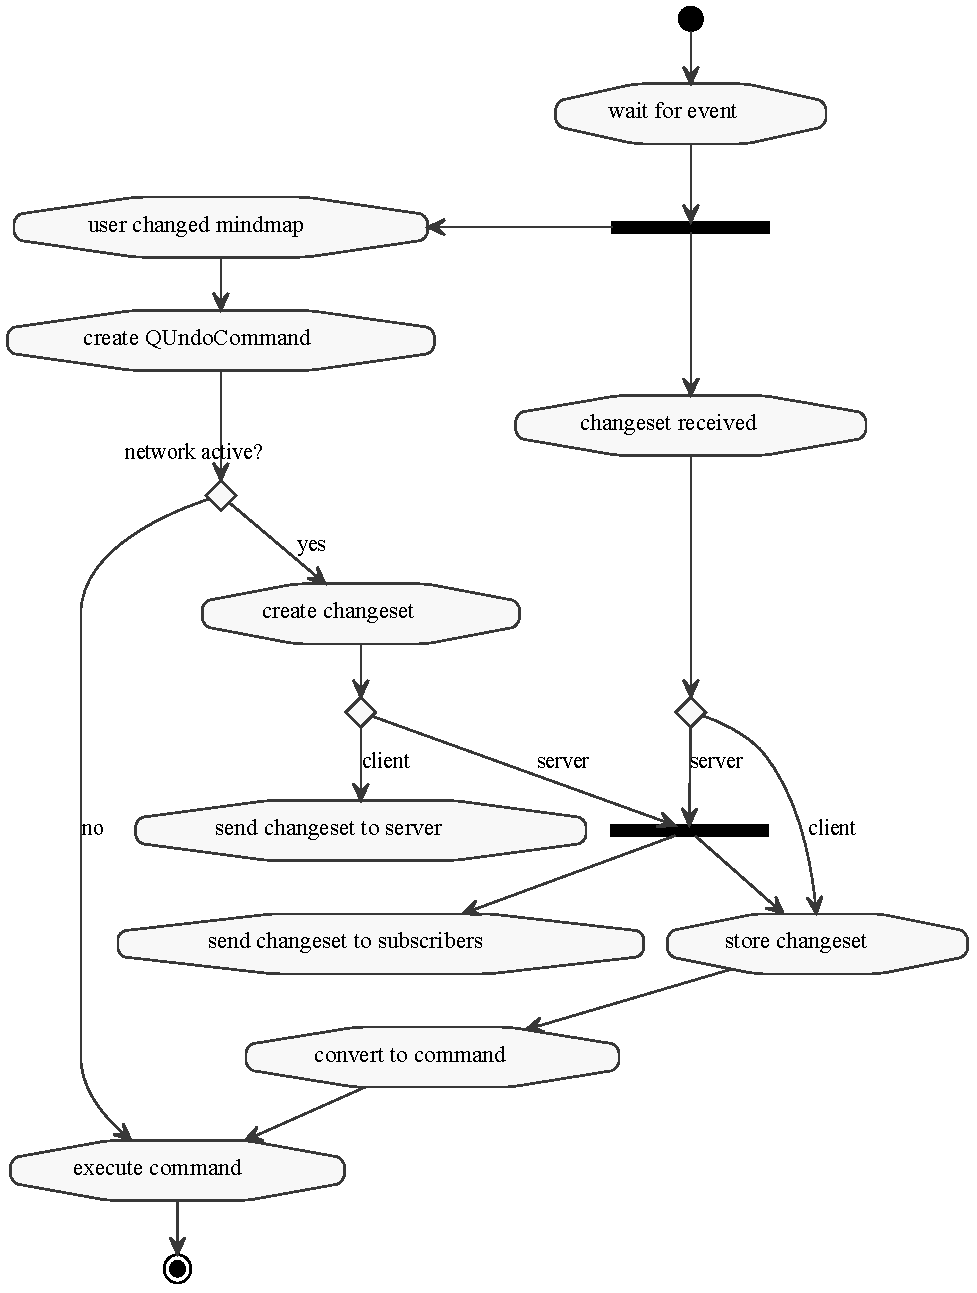
\includegraphics[width=\linewidth]{changeset-propagation.pdf}
  \caption{Диаграмма распространения изменений}
  \label{img:changeset_propagation}
\end{figure}

Для того чтобы управлять данным асинхронным взаимодействием был добавлен класс
NetworkController. Все команды поступают в сетевой контроллер. Если сетевое
взаимодействие неактивно, комманда добавляется в стек комманд. В противном
случае данная команда будет сериализована и отправлена на сервис. Уведомления
пришедшие от сервиса десериализуются в команды, добавляются в стек команд и
выполняются.

Данные команды содержат в себе информацию лишь об изменившейся части диаграммы.
Данное условие необходимо, чтобы уменьшить объём пересылаемых данных, который в
противном случае будет чрезмерно большим. Для того чтобы пересланная команда
выполнялась корректно у всех участников, необходимо чтобы они имели одинаковые
копии диаграмм. Поэтому встаёт вопрос о распространении и синхронизации
исходной диаграммы связи.

Проблема распространения диаграммы решается слеудующим образом: первый элемент в
узле должен содержать в себе сериализованную диаграмму связей. Все остальные
элементы содержат в себе сериализованные команды изменений. Когда участник
становится авторизованным подписчиком ему пересылаются все элементы содержащиеся
в узле, включая диаграмму и совершенные ранее изменения.

Синхронизация диаграммы связей между всеми участниками представляет более
сложную проблему. Фактически речь идёт о сохранение целостности диаграммы связи,
то есть контроле поступающих изменений. При поступлении некорректного изменения,
сервер должен отбросить изменение или провести слияние изменений, если возможно.
К примеру, из-за задержек в соединении пользователь может изменить узел, который
уже удалён одним из участников. В таком случае сервер должен отослать
пользователю уведомление об ошибке и отбросит некорректное изменение.

Подписчик может запросить все данные или часть данных, хранящихся в узле, в
любой момент времени. Данная возможность используется для синхронизации
локальной копии диаграммы в случае если изменение было отброшено сервером.
Сервер не нуждается в дополнительных способах синхронизации диаграммы, поскольку
все изменения локальны и всегда являются актуальными и корректными.

\section{Реализация сетевой подсистемы}
Сетевая подсистема приложения была реализована поверх фрэймворка Twisted и
библиотеки Wokkel. Wokkel является надстройкой над Twisted, добавляющей
фрэймворку дополнительную функциональность. В частности он предоставляет
средства для более удобной реализации XMPP расширений (XEP) и имеет поддержку
следующих: Service Discovery (XEP-0030), Publish-Subscribe (XEP-0060).
Реализация расширения публикации/подписки в Wokkel не содержит бизнес-логики.
Это значит, что он отвечает за приём, генерацию и отправку сообщений в
соответствии со спецификацией XEP-0060. Wokkel реагирует на события, относящиеся
к публикации/подписке, делает разбор пришедших сообщений и вызывает
соответствующие обработчики.

Расширение публикации/подписки является одним из самых больших и сложных.
Правильная реализация необходимого функционала может занять большое количество
времени. Поэтому было принято решение использовать библиотеку Idavoll. Данная
библиотека реализована поверх Wokkel и реализует функциональность XEP-0060
необходимую для приложения, такую как: ``Подписка'', ``Публикация'', ``Создание
узлов'', ``Хранилище элементов''. Также она имеет хорошую архитектуру,
позволяющую добавлять реализацию новой функциональности, определенной стандартом
расширения публикации/подписки. Idavoll имеет множество классов необходимых для
реализации спецификации XEP-0060 (см. рис. ~\ref{img:network_classes}).

Класс Node является абстрактным классом и представляют собой узел в терминах
XEP-0060. Существуют два типа узлов: LeafNode и CollectionNode. LeafNode может
содержать только элементы, когда как CollectionNode может содержать лишь другие
узлы. LeafNode хранит элементы в виде простого списка, но это не является
подходящим решением для приложения. Как было сказано в главе
~\ref{sec:changeset_propagation}, необходимо проверять приходящие изменения на
корректность. Для этого был создан класс Changeset, хранящий в себе информацию о
самом изменении, его типе, времени создания и авторе данного изменения. Также
создан специальный класс-контейнер СhangesetStack, хранящий экземпляры класса
Changeset и отвечающий за корректность и согласованность изменений находящихся в
нём. HivemindNode унаследован от LeafNode и в отличии от него хранит изменения в
ChangesetStack.

BackendService содержит реализацию бизнес-логики XEP-0060. В нем содержится
логика для работы с подписчиками, проверка прав доступа и т.д. Он связан
отношением композиции с классом Storage, отвечающим за управление узлами
(создание, удаление, конфигурирование). Класс HivemindNode, создаётся классом
Storage и содержит в себе методы для добавления данных, изменения конфигурации
узла, списка подписчиков и их ролей. PubSubService является классом библиотеки
Wokkel отвечающий за разбор пришедших сообщений и вызов соответствующих методов.
Если он содержит в себе экземпляр класса PubSubResourceFromBackend, то помимо
вызова своих обработчиков, осуществляется передача уже разобранных сообщений в
подходящие методы класса PubSubResourceFromBackend. Этот класс является
дополнительным уровнем абстракции, что позволяет делать архитектуру более
гибкой. PubSubResourceFromBackend обязательно содержит экземпляр класса
BackendService, которому он делегирует реализацию бизнес-логики.

\begin{figure}
  \centering
  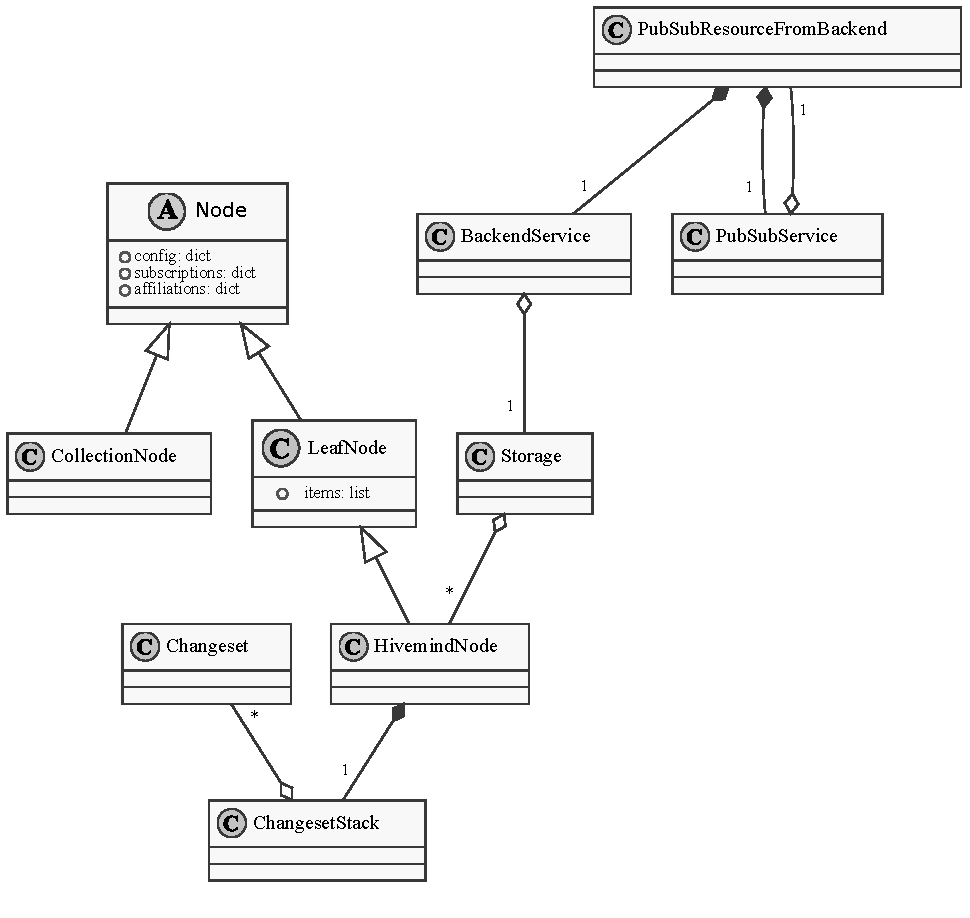
\includegraphics[width=\linewidth]{idavoll-classes.pdf}
  \caption{Диаграмма сетевых классов}
  \label{img:network_classes}
\end{figure}

Мобильные устройства зачастую имеют нестабильное соединение с сетью Интернет,
поэтому приложение должно иметь механизм, позволяющий обнаружить, что соединение
потеряно и уведомить об этом пользователя. Механизм проверки осуществляется
посредством XMPP Ping (XEP-0199) \cite{xep-0199}. Класс Pinger
ответственен за отсылку пинг сообщений и приём ответов. Проверка осуществляется
следующим образом: данный класс непрерывно отсылает пинг сообщения на XMPP
сервер, к которому подключен пользователь, если достигнуто определенное
количество пинг соббщений, оставшихся без ответа, то соединение рассматривается
как потерянное.

Похожий механизм используется для проверки статуса подписчиков. Каждый
подписчик имеет свой экземпляр класса Pinger, который отвечает за отсылку пинг
сообщений именно ему. На клиентской стороне реализован обработчик, который
отвечает на приходящие пинг сообщения от сервера приложения. Подписчиков может
быть очень много, поэтому был создан класс PingManager, отвечающий за управление
экземплярами класса Pinger (см. рис. ~\ref{img:ping_manager}). Он
создаёт и удаляет экземпляры класса Pinger, а также запускает или останавливает
отправку пинг сообщений до адресата. Pinger уведомляет NetworkController о
состоянии соединения с XMPP сервером, а также со всеми подписчиками.
Пользователь может увидеть статус соединения с подписчиками в диалоге
редактирования прав доступа(см. рис. ~\ref{img:permissions_dialog})

\begin{figure}
  \centering
  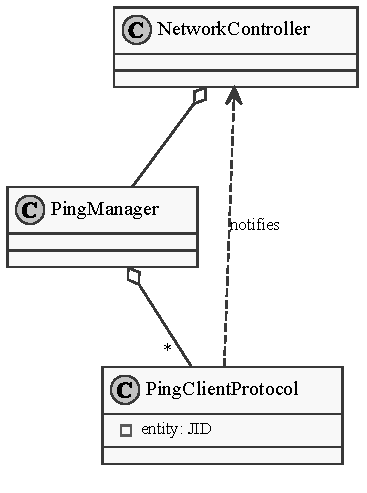
\includegraphics[scale=1.2]{ping-manager.pdf}
  \caption{Диаграмма классов, отвечающих за проверку состояния соединений}
  \label{img:ping_manager}
\end{figure}


\section{Система контроля доступа}

By default, all participants of teamwork have equal permissions to contribute to
the mind map. It is quite convenient for brainstorming-like activities when the
purpose of the collaboration is to generate some materials or to find a solution
for a long-standing problem. This kind of behavior looks unsuitable for other
use cases. Sometimes it is useful to restrict access for particular users in
order to prevent accidental interference of teamwork. To take such scenarios
into account we introduced access control system to HiveMind.

XEP-0060 provides a feature, named Access Model, which can be associated with
authentication system. The user, who creates the mind map, can set trust level
for all new participants i.e. control who can participate in collaboration.
There are four access models implemented in HiveMind:
\begin{itemize}
\item ``Open'' --- any person may join collaboration;
\item ``Roster'' --- only contacts from the owner’s roster may join;
\item ``Authorize'' --- the owner choose who may join on the fly. When a new
  person is connected, the owner gets a participation request from the person;
\item ``Whitelist'' --- a person may join only if he/she is in the owner’s
  whitelist.
\end{itemize}

``Affiliations'' is the next feature, defined in XEP-0060, being a part of
HiveMind access control system. This feature provides authorization capabilities
to XEP-0060. After the person joined collaboration, he/she has a role, which
determines a set of allowed actions. There are four roles implemented in
HiveMind:
\begin{itemize}
\item ``Outcast'' --- person not allowed to join collaboration i.e. in terms of
  IM he/she is banned;
\item ``Member'' --- person allowed to receive items;
\item ``Publisher'' --- person allowed to publish and receive items;
\item ``Owner'' --- similar to the Publisher, but allowed to configure
  collaboration behaviour.
\end{itemize}
Service owner can edit role of desired person at any time with the use of
permissions dialog (fig.~\ref{img:permissions_dialog}).

\begin{figure}[b] 
  \centering
  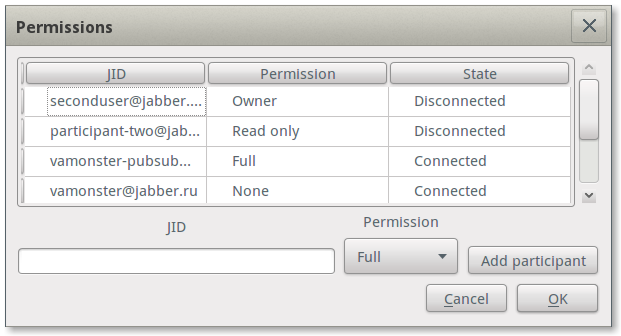
\includegraphics[width=0.5\linewidth]{permissions_dialog.png}
  \caption{Диалог управления правами доступа}
  \label{img:permissions_dialog}
\end{figure}

XEP-0060 has features that makes access control even more flexible. In some
cases it might be useful to temporarily assign publisher role to all
participants. HiveMind has implementation of XEP-0060 feature named Publish
Model. It determines two cases of who is allowed to make changes to the
mindmap. In the first case it is a person whose affiliation is publisher, and in
the second case any participant is allowed to post changes.

Impelementation of access control system helps us to discover new use cases of
HiveMind. Presentation using HiveMind is one of such use cases. First of all,
lecturer can control who may join the presentation. Secondly, there are can be
more than one lecturer. Presentations using HiveMind distinguish from
collaborative editing: lecturer's current node and fold/unfold events must be
propagated through the network. This ensured that participants can track the
presentation movement.
 
Authorization system can be extended to greatly improve presentation
support. For example, lecturer may want to receive questions. Participants
can add nodes containing a questions or suggestions to lecturer mindmap.
Authorization system controls interaction between lecturer and participants e.g.
participant is able to modify only his own nodes and not able to modify nodes
created by lecturer or other participants.
